\chapter{A Large Ion Collider Experiment at LHC}

\label{cap:3}


\vspace*{2cm}
\section{The Large Hadron Collider}
\label{par:3.1}
The Large Hadron Collider (LHC) is the world's largest and most powerful particle accelerator. It was inaugrated on 10 September 2008, and consists of a 27-kilometre ring of superconducting magnets with a number of accelerating structures to boost the energy of the particles along the way. By design, the maximum energies reached in the accelerator are \mbox{$7$ TeV} for a beam of protons and \mbox{$2.76$ TeV} per nucleon for a beam of lead ions, thus providing collisions at \mbox{$\sqrt{s}$ = $14$ TeV} and \mbox{$\sqrt{s_{NN}}$ = $5.5$ TeV}, respectively. During Run 2, LHC was able to reach \mbox{$13$ TeV} for pp and \mbox{$2.51$ TeV} for Pb-Pb collisions. and These are the largest energies ever achieved in particle collision experiments.


Inside the accelerator, two high-energy particle beams travel at close to the speed of light before they are made to collide. The beams travel in opposite directions in separate beam pipes - two tubes kept at ultrahigh vacuum. They are guided around the accelerator ring by a strong magnetic field maintained by superconducting electromagnets. The accelerator bends the beams around the ring, keeping the bunches focused and accelerate them to their collision energy. Finally, bunches are squeezed in order to ensure a high number of collisions per time interval at the collision points, i.e. a high luminosity\footnote{For a particle accelerator experiment, the luminosity is defined by: \mbox{$\mathcal{L} = fnN^{2}/A$} with $n$ number of bunches in both beams, $N$ number of particles per bunch, cross-sectional area $A$ of the beams that overlap completely, and revolution frequency $f$. The frequency of interactions (or in general of a given process) can be calculated from the corresponding cross-section $\sigma$ and the luminosity: \mbox{$dN/dt = \mathcal{L}\sigma$}.}. A combination of magnetic and electric fields components perform the mentioned tasks. Despite the high luminosity reached, only a very small fraction of the particles from the two bunches collide in a single bunch crossing. The others leave the interaction region essentially uninfluenced, and continue to circulate in the accelerator.


Injection of bunches into the LHC (\mbox{Figure \ref{Fig:cap3-1.1}}) is preceded by acceleration in the LINAC2, PS booster, PS, and SPS accelerators. The acceleration sequence is slightly different for heavy-ions, in which case bunches pass the LINAC3, LEIR, PS, and SPS accelerators. Several injections to the LHC are needed until all bunches of both beams are filled. The LHC produces collisions in four so called Interaction Points (IPs) in correspondence of which are located six detectors of different dimensions and with different goals, all able to study the products of the interactions. These are: 
\begin{itemize}
\item \textbf{ALICE (A Large Ion Collider Experiment - IP2):} is a dedicated heavy-ion experiment designed to study strongly-interacting matter at very high energy density. A detailed description of ALICE detector will be covered in the next section.

\item \textbf{ATLAS (A Toroidal LHC ApparatuS - IP1) and CMS (Compact Muon Solenoid - IP5):} are general-purpose detectors for pp collisions that are built to search for the Higgs boson and physics beyond the Standard Model, e.g. new heavy particles postulated by supersymmetric extensions (SUSY) of the Standard Model and evidence of extra dimensions. They have discovered the Higgs boson in 2012. 

\item \textbf{LHCb (The Large Hadron Collider beauty experiment - IP8):} is a dedicated experiment to study heavy flavour physics at the LHC. The experiment complements the studies conducted at B-factories and the search for new particles at ATLAS and CMS. 
\item \textbf{LHCf (Large Hadron Collider forward experiment - IP1):} is placed closed to the ATLAS experiment and studies the forward particles created during LHC collisions.

\item \textbf{TOTEM (TOTal Elastic and diffractive cross-section Measurement - IP5):} is located close to the CMS detector and measures the total cross-section, elastic scattering, and diffractive processes.

\end{itemize}


\begin{figure}[t]
\centering
\includegraphics[width=1.0\textwidth]{Images/Cern-Accelerator-Complex}
\caption[The CERN accelerator complex.]{The CERN accelerator complex.}
\label{Fig:cap3-1.1}
\end{figure}

\subsection{The LHC as a heavy-ion accelerator}
\label{par:3.1a}
\textbf{OPTIONAL SECTION}
Since its early stages, LHC was designed to perform as well as heavy ion collider, in particular to feed ALICE with data, although also CMS and ATLAS included the study of ion collisions with similar luminosities in their physics program.\footnote{LHCb did not participate in the Pb-Pb run in 2010 and 2011.}
\\
The source of Pb ions is a 3 cm lead cylinder heated to about 500 C. This vaporises a small amount of atoms, that once partially ionised by strong electrical fields are accelerated in a linear device to strip the remaining electrons to create $^{208}Pb^{82+}$ ions. These ions are then injected and accumulated in Low Energy Ion Ring (LEIR) and then sent to the Proton Synchrotron (PS). Further on, they follow the same injection procedure as protons. The ions can reach a centre of mass  energy of 5.5 TeV/ nucleon or a total centre of mass energy of 1.15 PeV with the nominal magnetic field of 8.33 T in the dipole magnets. 

\section{The ALICE Detector}
\label{par:3.2}
ALICE (A Large Ion Collider Experiment) is a general-purpose, heavy-ion detector at the LHC which focuses on Quantum Chromodynamics, the strong-interaction sector of the Standard Model. It has been collecting data since the beginning of LHC operations in 2008 and will continue to do so until the end of 2018 for the planned long shutdown. During the first three years of operations LHC provided pp collisions at 0.9, 2.76, 7and 8 TeV, Pb-Pb collisions at 2.76 TeV and finally p-Pb collisions at 5.02 TeV and in the second phase, LHC reached close to it's designed maximum energies at 13 TeV for pp, and 5.02 TeV for Pb-Pb and 8 TeV at p-Pb collisions.It has been designed to study the physics of strongly interacting matter and the quark-gluon plasma at extreme values of energy density and temperature in nucleus-nucleus collisions. ALICE allows for a comprehensive study of hadrons, electrons, muons, and photons produced in the collision of heavy nuclei (Pb-Pb), up to the highest multiplicities at the LHC. The physics programme also includes analysing proton-proton and proton-nucleus collisions to address various QCD topics. The detector, located at the interaction point 2 along the LHC ring, has been designed to cope with a high particle multiplicity environment and to provide unique particle identification (PID) performance that allow a comprehensive study of hadrons, electrons, muons, and photons produced in the collision, down to very low transverse momentum (0.1 \GeVc). \mbox{Figure \ref{Fig:cap3-1.2}} shows the ALICE detector schema and \mbox{Figure \ref{Fig:cap3-1.3}} shows the cross section of the central barrel. The central barrel covers a mid rapidity region $|\eta| < 0.9$ and azimuthal range of $2\pi$. 

\begin{figure}[t]
\centering
\includegraphics[width=1.0\textwidth]{Images/Chapter3/detALICE}
\caption[The ALICE detector]{The ALICE detector}
\label{Fig:cap3-1.2}
\end{figure}


\begin{figure}[t]
\centering
\includegraphics[width=1.0\textwidth]{Images/Chapter3/cross_section}
\caption[Cross Section of Central Barrel of ALICE]{Cross Section of Central Barrel of ALICE}
\label{Fig:cap3-1.3}
\end{figure}

The central barrel of the detector is enclosed in L3 solenoid magnet which provides a 0.5 T magnetic field, and is followed by a forward muon spectrometer which has its own dipole magnet providing a field of 0.67 T. The central barrel consists of, going from beam pipe outwards, a six layer Inner Tracking System (ITS) that provides precise tracking and vertex reconstruction, a large volume Time Projection Chamber (TPC) which is responsible for global tracking and particle identification (PID) through the measurement of specific energy loss in a gas, a Transition Radiation Detector (TRD) allowing for identification of electrons and the outermost of the central barrel is a Time of Flight detector (TOF) which allows for identification of charged hadrons. \\
\\TRD covers full azimuth of the mid-rapidity region ($-0.84 < \eta < 0.84$) from 2.90 m to 3.68 m from the interaction vertex. It has the main task to provide electron identification in the ALICE central barrel for particle momenta greater than 1 \GeVc. Electrons with momentum above this value radiate transition radiation \footnote{Transition radiation is produced by relativistic charged particles ($\gamma \geq 1000$) when they cross the interface of two media of different dielectric constant. Photons are emitted in the $keV$ range with typical energy $$\hbar\omega \approx \frac{1}{4}\hbar\omega_{p}\gamma ,$$ where $\omega_{p}$ is the plasma frequency $$\omega_{p} = \sqrt{\frac{n_{e}e^{2}}{\epsilon_{0}m_{e}}}$$ where $n_{e}$ is the electron density} which can be exploited to extend the pion rejection capability of the TPC to higher momenta. Furthermore, the TRD provides tracking information with a larger tracking lever arm, thus improving momentum resolution at high \pT. The detector can also derive a fast trigger for high-momentum charged particles and it contributes to the Level-1 trigger of ALICE.

The detectors which are important to this work will be explained in the following sections (namely TPC, ITS, TOF and VZERO)\\
\\

Besides the aforementioned detectors, the following detectors located inside the L3 magnet provide limited acceptance, outside the TOF: 
\begin{itemize}
\item \textbf{HMPID}: High Momentum Particle Identification detector is a dedicated detector for inclusive measurements of identified hadrons at \pT >1 \GeVc.  It is based on proximity-focusing Ring Imaging Cherenkov (RICH) counters \footnote{Cherenkov radiation is emitted when a charged particle passes a dielectric medium with velocity $$\beta \geq \beta_{thr} = 1/n$$, 
 where $n$ is the refractive index of the medium. The photons are emitted at an angle $$cos\theta_{c} = \frac{1}{n\beta}$$} arranged in an array with an acceptance of $5\%$ of the central barrel phase space with the aim of enhancing the PID capability of ALICE by enabling identification of charged hadrons beyond the momentum interval attainable through energy-loss (in ITS and TPC) and time-of-flight measurements (in TOF). Identification of light nuclei and anti-nuclei ($d$, $t$, $^{3}$He, $\alpha$) at high transverse momenta in the central rapidity region can also be performed with the HMPID. 

\item \textbf{Calorimeters}
\begin{enumerate}}

\item \textbf{EMCal/DCal:} The aim of ElectroMagnetic Calorimeter and Di-Jet Calorimeter is to enable ALICE to measure jet properties and providing trigger on jets and high momentum photons and electrons. The EMCal and DCal are  large Pb-scintillator sampling calorimeters with cylindrical geometry, located adjacent to the ALICE magnet coil at a radius of $\sim$ 4.5 metres from the beam line. EMCal subtends $110^{\circ}$ and the DCal subtends $60^{\circ}$ in $\phi$, with both detectors covering $|\eta| < 0.7$, thereby providing good acceptance for di-jets with $R\leq 0.4$ up to transverse momenta $\pT \sim 150 \GeVc$

\item \textbf{PHOS}: Photon Spectrometer is a high-resolution electromagnetic calorimeter which detects electromagnetic particles in a limited acceptance region at central rapidity to provide photon identification as well as neutral-meson reconstruction through the 2-photon decay channel. It's main physics objectives are the test of thermal and dynamical properties of the initial phase of the collision extracted from low \pT direct photon measurements and the study of jet quenching through the measurement of high-\pT $\pi^{0}$ and $\gamma$-jet correlations. It is positioned at a distance of 460 cm from the interaction point, azimuthally opposed to the EMCAL, and covers a limited acceptance ($|\eta| < 0.12$ and $\Delta \phi =100^{\circ}$ ).

\end{enumerate} 

\end{itemize}

In addition to the central barrel detectors described above, ALICE has a dedicated Muon Spectrometer, a set of forward detectors and ACORDE.

\subsection*{\textbf{Muon Spectrometer}}
This detector, placed in the forward pseudo-rapidity region ($-4.0 < \eta < -2.5$), consists of a dipole magnet and tracking and trigger chambers. It is optimised to reconstruct heavy quark resonances (such as $J/\Psi$ through their $\mu^{+}\mu^{-}$ decay channel) and single muons

\subsection*{\textbf{Forward Detectors}}
They are placed in the high pseudo-rapidity region (small angles with respect to the beam pipe) they are small and specialised detector systems used for triggering or to measure global event characteristics. 
\begin{itemize}
\item Time Zero (T$0$) to measure the event time with precision of the order of tens of picoseconds, as needed by TOF
\item VZERO to reject the beam-gas background and to trigger minimum bias events
\item Forward Multiplicity Detector (FMD) to provide multiplicity information over a large fraction of the solid angle ($-3.4 < \eta < -1.7$ and $1.7 < \eta < 5$)
\item Photon Multiplicity Detector (PMD) to measure the multiplicity and the spatial distribution of photons on an event-by-event basis in the $2.3 < \eta < 3.7$ region
\item Zero Degree Calorimeter (ZDC) to measure and trigger on the impact parameter. The ZDC consists of two calorimeters, one for neutrons (ZDC:ZN) and one for protons (ZDC:ZP), and includes also an electromagnetic calorimeter (ZEM).
\end{itemize}

\subsection*{\textbf{ACORDE}}
ACORDE is an array of scintillators installed on top of the L3 magnet to trigger on cosmic rays.


\subsection{Inner Tracking System}
\label{par:3.2a}
ITS is the main detector responsible for measuring the primary vertex of the collisions being the innermost tracking detector closest to the beam pipe. It has 6 layers of concentric cylindrical detectors based on three different technologies of silicon detectors : pixels, drifts and strips (\mbox{Figure \ref{Fig:cap3-1.4}}).  It is positioned at radius between 4 and 43 cm, surrounding the LHC beryllium beam pipe that is 800μm thick and has a radius of 2.9 cm. \\

\begin{figure}[t]
\centering
\includegraphics[width=0.8\textwidth]{Images/Chapter3/its}
\caption[Inner Tracking System]{The Inner Tracking System of ALICE}
\label{Fig:cap3-1.4}
\end{figure}

The two innnermost ITS layers constitute the SPD, Silicon Pixel Detector. A total of $9.8 x10^{6}$ readout channels receive signals from the 20 half-staves of the SPD, each of them consisting of 240 modules with 1200 readout chips. Thanks to the high-granularity the SPD has also been used for the trigger system, especially for the minimum bias event selection. The SPD is mainly used to determinate the primary vertex position, with a resolution of the order of $100 \mu m$.\\
\\
The Silicon Drift Detector (SDD) is based on modules with a sensitive area of 70.17 ($r\phi$) x 75.26 ($z$) $mm^2$, divided into two drift regions where electrons move in opposite directions under a drift field of approximately 500 $V/cm$. The SDD modules are mounted on a linear structure called ladder. The SDD inner layer is made of 14 ladders with 6 modules each, the outer layer has 22 ladders, each of them with 8 modules. The position of the particle along $z$ is reconstructed from the centroid of the collected charge along the anodes, while the position along the drift $r$ coordinate is obtained from the measured drift time with respect to the trigger time. This reconstruction requires a precise knowledge of the drift speed, that is measured during frequent calibration runs, given its strong dependence from the humidity and temperature gradients in the SDD volume.\\
\\
The Silicon Strip Detector (SSD) building block is a module composed of one double-sided strip detector connected to two hybrids hosting the front-end electronics. The sensors are 300 $\mu m$ thick and with an active area of 73 ($r$) x 40 ($z$) $mm^2$. There are 768 strips, with a pitch of 95 $\mu m$ on each side, almost parallel to the $z$ beam axis direction. The innermost SSD layer consists of 34 ladders, each of them housing 	22 modules along the beam direction, while the other SSD layer has 38 layers, each of them with 25 modules. The outer four layers are used particle identification via energy loss (dE/dx) measurement in the non-relativistic region for low momentum particles (down to \pT~=100 MeV) via analogue readout. \mbox{Figure \ref{Fig:cap3-1.5}} shows an example of the particle identification capabilities of the ITS for pp collisions at $B= 0.2 T$. The resolution in the $r\phi$ plane is nearly 50 $\mu m$ for 1 \GeVc particles and decreases at higher momentum. Resolution in Pb-Pb collisions is slightly better with respect to pp, as the high multiplicity of central Pb-Pb collisions implies a better primary vertex resolution.

MATERIAL BUDGET REDUCTION AND IMPACT PARAMETER RESOLUTION FOR CHARM RECON
\begin{figure}[t]
\centering
\includegraphics[width=0.8\textwidth]{Images/Chapter3/dEdx_13TeV}
\caption[dE/dx distribution of charged particles as function of their momentum, both measured by the ITS alone, in pp collisions at 13 TeV. The lines are a parametrization of the detector response based on the Bethe-Bloch formula.]{dE/dx distribution of charged particles as function of their momentum, both measured by the ITS alone, in pp collisions at 13 TeV. The lines are a parametrization of the detector response based on the Bethe-Bloch formula.}
\label{Fig:cap3-1.5}
\end{figure}

\subsection{The Time Projection Chamber}
\label{par:3.2b}
The Time Projection Chamber (TPC) is the main tracking detector of ALICE covering the pseudorapidity range $|\eta| < 0.9 $ and the full azimuth angle. The optimisation of the detector design has been done to provide excellent tracking performance in a high multiplicity environment, to keep the material budget as low as possible in order to have low multiple scattering and secondary particle production, to limit the detector occupancy at the inner radius but still guarantee a good momentum resolution for high–\pT~ particles. TPC is cylindrical in shape 500 cm long along the beam pipe, with 80 cm and 250 cm inner and outer radii respectively, determined by maximum acceptable track density and  minimum track length for which the resolution on dE/dx is lower than $10\%$. The TPC volume was filled with 90 $m^3$ of a mixture of Ne/$CO_{2}$/$N_{2}$ during Run 1, optimised for drift velocity, low electron diffusion and low radiation length. Neon was replaced by Argon for the second run. The electron drift velocity of 2.7 $cm/s$ over 250 $cm$ (each of the two TPC drift region separated by the central cathode) gives a maximum drift time of 88 $\mu s$, therefore limiting the maximum event rate TPC can sustain. At high interaction rate, pile-up effects and the long TPC dead time are the two main factors that force ALICE to run at a lower instantaneous luminosity with respect to the other LHC experiments. \\
\\
The TPC is able to track particles in a wide momentum range, from about \pT $\sim 0.1$ \GeVc~ up to \pT$\sim 100$ \GeVc~ with good momentum resolution and efficiency $>90\%$ for \pT$ > 100$ \MeVc, where the limiting factor are the interactions in the ITS material. The ITS and the TPC are able to determine the momentum of the charged particles with a resolution better than $1\%$ at low \pT and better than $20\%$ for \pT$\sim 100$ \GeVc (see \mbox{Figure \ref{Fig:cap3-1.6}}) by measuring the deflection in the magnetic field.\\

\begin{figure}[t]
\centering
\includegraphics[width=0.8\textwidth]{Images/Chapter3/tpcits_perf}
\caption[Momentum resolution for TPC-ITS]{Momentum Resolution for TPC-ITS}
\label{Fig:cap3-1.6}
\end{figure}



The charge collected in the TPC readout pads is used to measure particle energy loss. The momentum measurement and the dE/dx information allow to separate the various charged particle species in the low momentum region: thanks to its good dE/dx resolution, the TPC can identify particles with \pT$<1$ \GeVc. An example of the TPC PID performance is shown in \mbox{Figure \ref{Fig:cap3-1.7}}, where the energy loss distribution for the different species is fitted by a Bethe-Bloch function, similarly to the ITS case.

\begin{figure}[t]
\centering
\includegraphics[width=0.8\textwidth]{Images/Chapter3/tpc_dEdx_13TeV}
\caption[Energy loss in TPC in pp collisions at $\sqrt{s} = 13$TeV]{Energy loss in TPC in pp collisions at $\sqrt{s} = 13$TeV}
\label{Fig:cap3-1.7}
\end{figure}



\subsection{The Time of Flight Detector}
\label{par:3.2c}
TOF plays a key role in particle identification in the pseudorapidity region $|\eta| < 0.9$, by combining the measurement of the particle time-of-flight with the momentum information provided by the TPC. TOF is a large MRPC (Multi Resistive Plate Chamber) array located in the ALICE central barrel at a distance of 3.7 m from the beam line, externally to the TRD. The intrinsic time resolution of the MRPC is lower than 50 ps (from test beam studies) and it is dominated by the jitter in the electronics and the time resolution of the TDCs. The MRPC efficiency was measured to be close to $100\%$.  The design of TOF is optimised to minimise the dead zones and to be perpendicular to the trajectories of the particles coming from the IP, so to limit the occupancy and reduce the time resolution. The TOF detector consists of 152928 readout channels (2.5 x 3.5 $cm^2$ each) covering a total area of 141 $m^2$. This highly segmented structure allow to have a low occupancy and good performance also in a high multiplicity environment, such that of Pb–Pb collisions. An example of TOF performance is shown in \mbox{Figure \ref{Fig:cap3-1.8}}.

\begin{figure}[t]
\centering
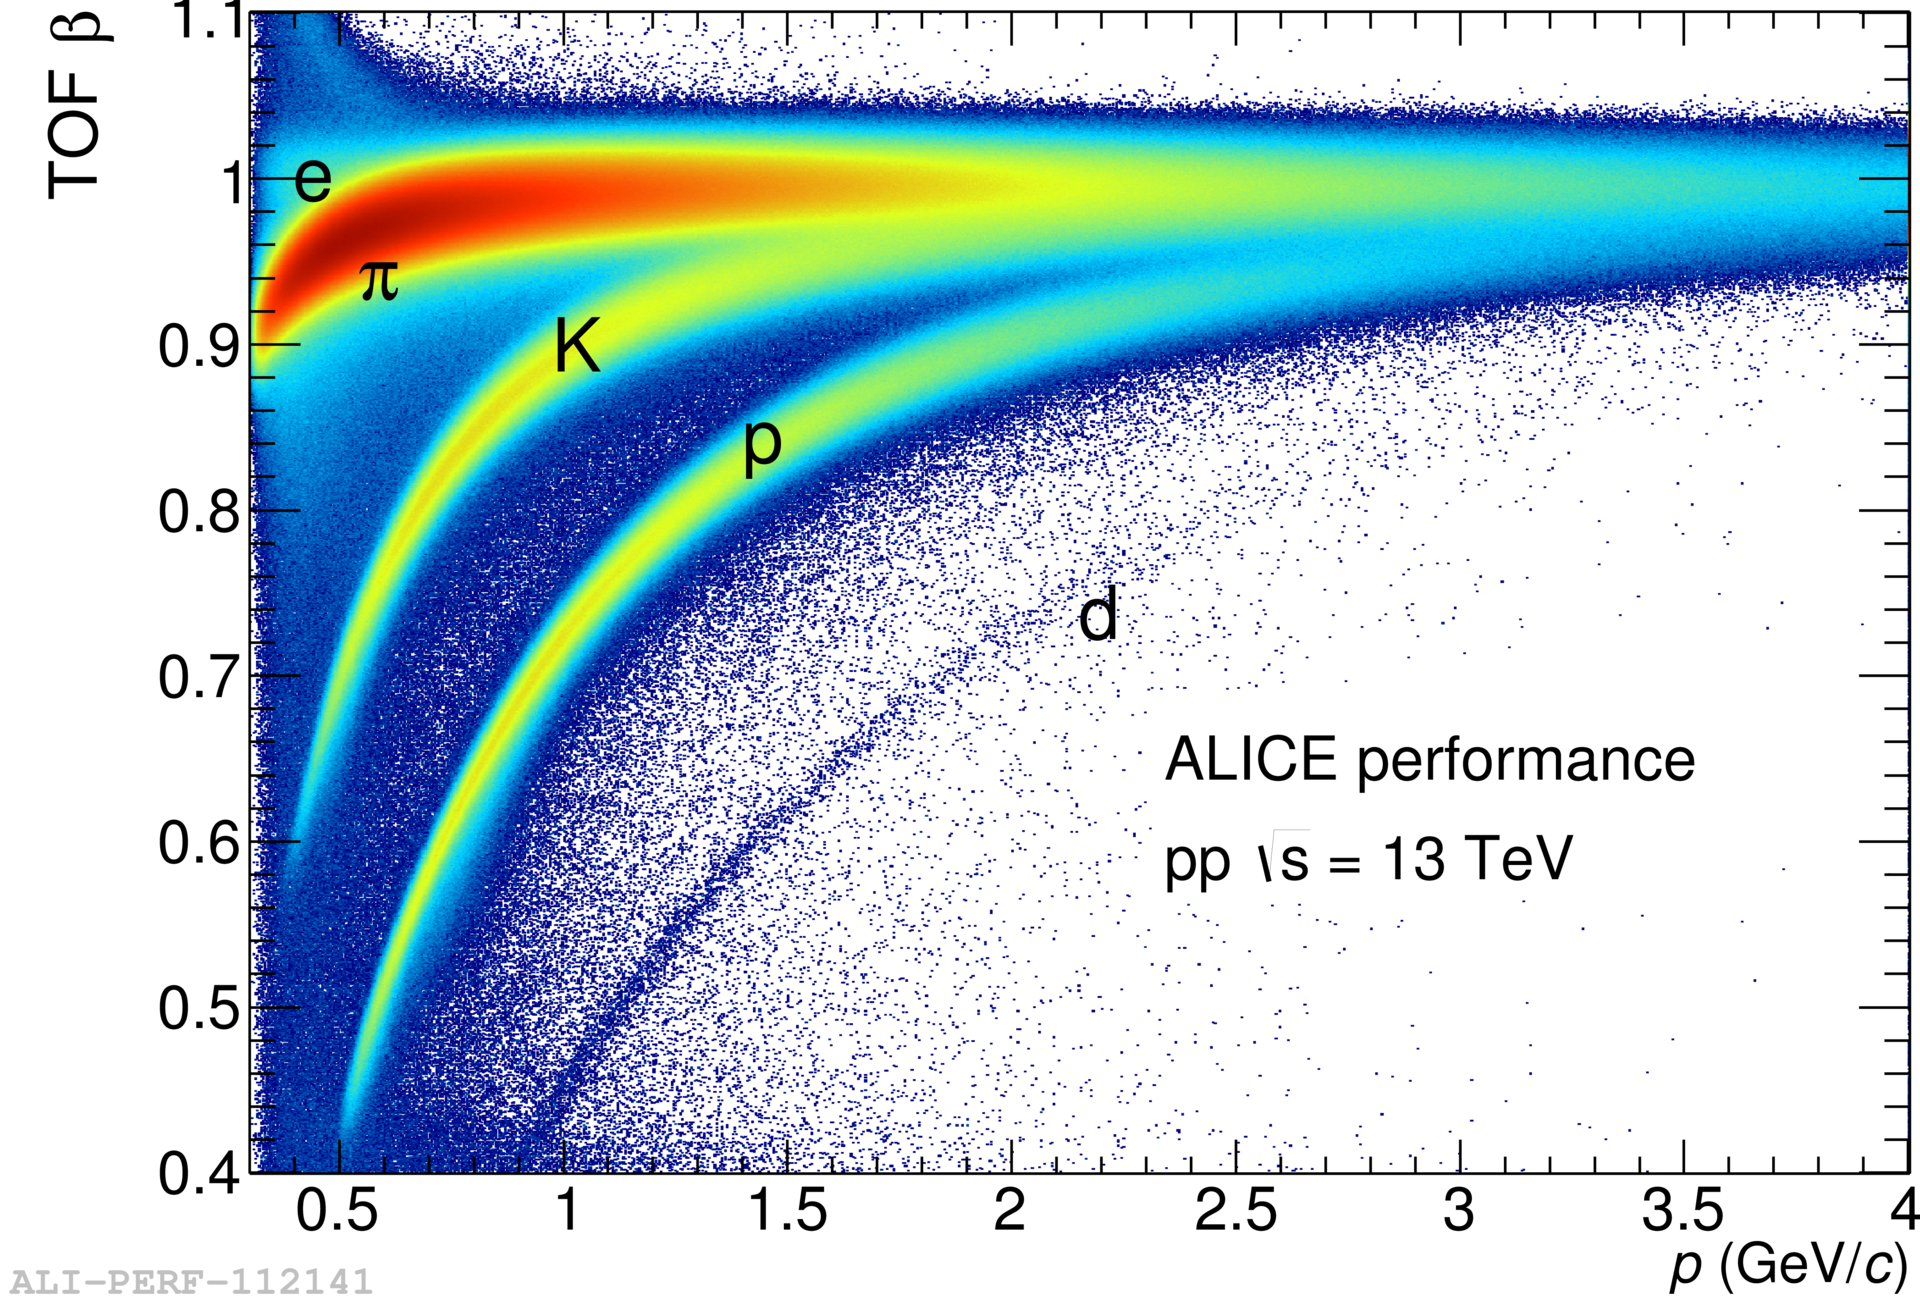
\includegraphics[width=0.8\textwidth]{Images/Chapter3/tof_beta}
\caption[TOF $\beta$ vs \pT performance plot in pp collisions at $\sqrt{s} = 13$TeV]{TOF $\beta$ vs \pT performance plot in pp collisions at $\sqrt{s} = 13$TeV}
\label{Fig:cap3-1.8}
\end{figure}

\subsection{VZERO}
\label{par:3.2c}
The VZERO is a trigger detector that provides a minimum-bias trigger for all colliding systems to the central barrel detectors and three centrality triggers in Pb–Pb collisions (multiplicity, central and semi-central). It has an important role in rejecting background from beam-gas collisions exploiting the relative time-of- flight measurement between the two arrays: when the beam-gas collision takes place outside the region between the two arrays, particles arrive 6 ns before or after the time of a beam-beam collision. It consists of two segmented arrays of plastic scintillator counters, called VZERO-A and VZERO-C, placed around the beam-pipe on either side of the IP: one at $z =$  340 cm, covering the pseudo-rapidity range, 2.8 $< \eta< $5.1, and the other at $z$ = -90 cm (in front of the absorber), covering the pseudo-rapidity range, -3.7$ < \eta <$ -1.7




\subsection{Data Acquisition (DAQ) and Trigger systems }
\label{par:3.2b}

\subsubsection*{Trigger System}
The ALICE Central Trigger Processor (CTP) has been designed to select events having a variety of different features at rates which can be scaled down to suit physics requirements and restrictions imposed by the bandwidth of the Data Acquisition (DAQ) system and the High-Level Trigger (HLT). Since the counting rates for different running modes (pp, pA, AA) can vary for almost two orders of magnitude, the biggest challenge for the ALICE trigger is to make optimum use of the detectors and to perform trigger selections in an optimised way for these different modes.\\
\\
The first response of the trigger system has to be fast to suit detector requirements. The “fast” part of the trigger is split into two levels: a Level-0 (L0) signal from CTP reaching the detectors after 1.2 $\mu s$ and a Level-1 (L1) signal arriving after 6.5 $\mu s$. The L0 signal is too fast to enable the trigger inputs from all the detectors while the L1 signal can pick up all the remaining fast inputs. CTP decisions are made in 100 $ns$.


\subsubsection*{Data Acquisition (DAQ)}
The trigger and Data Acquisition (DAQ) systems of ALICE have been designed to give different observables a fair share of the trigger and DAQ resources with respect to DAQ bandwidth. They have also to balance the capacity to record Pb-Pb central collisions (which generate large events) with the ability to acquire large fractions of rare events. To provide adequate physics statistics it has been estimated that a bandwidth of 1.25 $GB/s$ to mass storage is suitable. This bandwidth is consistent with constraints imposed by technology, cost and storage capacity.\\
\\
The architecture of the data acquisition is shown in \mbox{Figure \ref{Fig:cap3-1.9}}. Detectors receive the trigger signals from CTP (Central Trigger Processor) through LTU (Local Trigger Unit). The data produced by the detectors are injected on the DDL (Detector Data Link) using the same protocol. At the receiving end of the DDL, D-RORC (DAQ Readout Receiver Card) PCI-X based cards receive and assemble the event fragments into sub-events in the LDCs (Local Data Concentrators). The role of the LDC is to ship the sub-events to a farm of machines (Global Data Concentrator, GDC) where the whole events are built. The GDCs feed the recording system which eventually records the events in the Permanent Data Storage (PDS).

\begin{figure}[t]
\centering
\includegraphics[width=0.8\textwidth]{Images/Chapter3/alice_daq}
\caption[ALICE DAQ system]{The overall architecture of the ALICE DAQ system and the interface to the HLT system}
\label{Fig:cap3-1.9}
\end{figure}


\subsubsection*{High Level Trigger (HLT)}
According to the simulation studies, the amount of data produced in the TPC alone, in a single central nucleus-nucleus collision, corresponds to about 75 MB assuming $dN_{ch}/d\eta = 8000$ at mid- rapidity. The data rate for all detectors, resulting after a trigger selection, can easily reach 25 GB/s, while archiving rate is about 1 $GB/s$. Therefore online processing is advisable to select relevant events and to compress data without loosing their physics content. The overall physics requirements of the HLT are the following:
\begin{itemize}
\item \textbf{Trigger} Accept or reject events based on detailed online analysis
\item \textbf{Select} Select a physics region of interest within the event by performing only a partial readout
\item \textbf{Compress} Reduce the event size without loss of physics information by applying compression algorithms on the accepted and selected data
\end{itemize}



\subsection{Data flow: from the Online to the Offline }
\label{par:3.2c}
Several stages of processing of raw data taken by detectors before it is available in form of reconstructed events is depicted in \mbox{Figure \ref{Fig:cap3-1.10}}.

\begin{figure}[t]
\centering
\includegraphics[width=0.8\textwidth]{Images/Chapter3/data_flow}
\caption[ALICE Data Flow]{Global view of ALICE’s data flow}
\label{Fig:cap3-1.10}
\end{figure}

Data originating from the detectors (denoted by 1 in \mbox{Figure \ref{Fig:cap3-1.9}}) is processed by LDCs and global events are built by GDCs (2), as already mentioned. The so-called publish agent registers the assembled events into the AliEn system (3) and ships them to the CERN computing centre where they are stored first on disks (4) and then permanently on tapes (5) by the CASTOR system.\\
\\
During data-taking the detectors also produce conditions data that are relevant for the calibration of individual detector signals. Conditions data provide information about the detector status and environmental variables during data-taking. Examples are inactive and noisy channel maps, distributions that describe the response of a channel, temperatures and pressure in a detector, and detector configuration. Many of the conditions data could in principle be calculated from the raw data and extracted offline after data-taking. However, such an approach would require an additional pass over the raw data before the reconstruction which is not feasible due to the limited computing resources. Therefore, conditions data are already extracted during data-taking and stored in the Offline Condition Data Base (OCDB). A dedicated program called Shuttle collects these outputs and makes them available to the reconstruction. Furthermore, it retrieves information about the run from the ECS \footnote{The Experiment Control System (ECS) is the top level control of the ALICE experiment. Running an experiment implies performing a set of activities on the online systems that control the operation of the detectors. These online systems are: the Trigger (TRG), the Detector Control Systems (DCS), the Data-Acquisition System (DAQ) and the High-Level Trigger (HLT). The ECS provides a framework in which the operator can have a unified view of all the online systems and perform operations on the experiment seen as a set of detectors.} logbook (9) and collects continuously monitored values that are written by DCS into the DCS Archive (10). After processing the data, the Shuttle registers the produced condition files in AliEn (11) and stores the data in CASTOR (12).\\
\\
With the registration of the raw and conditions data the transition from the online to the offline world has taken place. "Online" denotes all actions and programs that have to run in real time. "Offline" processing is the subsequent step, like for instance the event reconstruction, which is executed on worker nodes (WN) of Grid sites located around the Globe.



\subsection{ALICE Offline software framework }
\label{par:3.2d}
The required computing resources for the reconstruction and analysis of the raw data, as well as the production of simulated events needed for the understanding of the data, exceed the computing power of single institutes and even centres like CERN. Therefore, institutes that are part of the Collaboration provide storage and computing resources. Distribution of the data for reconstruction and analysis cannot be performed manually leading to the need for an automated system. The concept of a decentralised computing model called Grid was identified as a solution.

\subsubsection{The AliEn Framework}
The Grid unifies the resources of distributed computing centres, in particular computing power and storage, to provide them to users all over the World. It allows computing centres to offer their resources to a wider community, and the local resources to be shared by an entire collaboration.\\
\\
Software that implements the Grid concept is called Grid middleware. Since 2001ALICE has developed a Grid middleware called AliEn. An ALICE user employs AliEn to connect to the ALICE Grid which is composed of a combination of general services that are provided by many Grid middleware solutions and ALICE-specific services provided by AliEn. Parts of the ALICE Grid are:
\begin{enumerate}
\item a global file catalog that is a directory of files in storage elements distributed over the globe
\item  the automatic matching of jobs for execution to a suitable location in one of the connected sites
\item  a shell-like user interface 
\item API9 services for the ROOT framework
\end{enumerate} 
Currently the ALICE Grid consists of about 130 sites located in 21 countries. \mbox{Figure \ref{Fig:cap3-1.11}} shows a map of the ALICE Grid sites.

\begin{figure}[t]
\centering
\includegraphics[width=0.8\textwidth]{Images/Chapter3/grid_sites}
\caption[ALICE Grid sites]{ALICE Grid sites}
\label{Fig:cap3-1.11}
\end{figure}

\subsubsection*{The AliRoot Framework}
AliRoot is the offline framework for simulation, alignment, calibration, reconstruction, visualisation, quality assurance, and analysis of experimental and simulated data. It is based on the ROOT framework. Most of the code is written in C++ with some parts in Fortran that are wrapped inside C++ code. Re-usability and modularity are the basic features of the AliRoot framework. Modularity allows parts of the code to be replaced, with minimum or no impact on the rest (for example changing the event generator, the transport Monte Carlo or the reconstruction algorithms) which is achieved by implementing abstract interfaces. In addition codes for each detector subsystem are independent modules with their specific code for simulation and reconstruction, which can be developed concurrently with minimum interference. Re-usability is meant to maintain a maximum amount of backward compatibility as the system evolves.\\
\\
The central module of the AliRoot framework is STEER (\mbox{Figure \ref{Fig:cap3-1.12}}) which provides several common functions such as steering of program execution for simulation, reconstruction and analysis; general run management; creation and destruction of data structures; initialisation and termination of program phases; base classes for simulation, event generation, reconstruction, detectors elements. For event simulation the framework provides the following functionality:

\begin{itemize}
\item \textbf{Event Generation:} Many MC event generators (e.g. Pythia, Phojet, EPOS for pp events and HIJING for Pb-Pb events) are interfaced with AliRoot. For each generated particle a list of information (such as type, momentum, charge, production process, originating particle and decay products) is stored in a file (kinematics tree).

\item \textbf{Transport:} The detector structure, the motion of the particles through it and the possible interactions with the material are simulated using programs such as Geant3, Geant4 and Fluka. For all the interactions of particles with sensitive parts of the detector (hits), information such as position, time, energy deposition and the tag of track they belong to, are recorded during this process

\item \textbf{Digitisation:} Finally all the hits are translated in the corresponding digital output of the detector, taking into account the detector's response function. All this information are then stored in the specific hardware format of the detector (raw data).
\end{itemize}


\begin{figure}[t]
\centering
\includegraphics[width=0.8\textwidth]{Images/Chapter3/STEER}
\caption[AliRoot framework]{Schema of the AliRoot framework}
\label{Fig:cap3-1.12}
\end{figure}

\subsection{Event reconstruction }
\label{par:3.2e}
At this stage the raw data correspond to the signals that would have been produced by an interaction of the same kind within the detector. The subsequent reconstruction is identical, both for simulated as well as real events. It consists of the following steps:

\begin{itemize}
\item \textbf{Cluster Finding:} Usually, particles that interact with a detector, depending on its spatial segmentation, leave a signal in several adjacent detecting elements. Similarly a signal, last in a time interval can be distributed on more than one time bin. The first required step in the event reconstruction is the cluster finding, i.e  the construction of sets of spatial or time close signals that reduce the effect of random noise in the position or timing measurement.

\item \textbf{Track Reconstruction:} The tracking is a complex and iterative procedure that, starting from clusters, uses the Kalman filter technique to follow inward and outward the track fitting. The tracking is a global task as well as a set of detector-specific procedures. The different steps of the global track reconstruction are schematically reported in \mbox{Figure \ref{Fig:cap3-1.13}}. The procedure starts from track "seeds" in the outermost part of the TPC, which are selected under the assumption that the corresponding track originated from the primary vertex. Than the TPC only reconstruction ends with a similar seeding in the innermost part of the TPC, the removal of all the clusters already associated to tracks and the final filtering which is performed without requiring that the seeds point to the primary vertex. Subsequently, these tracks are complemented with information from the ITS, TRD, and TOF as well as HMPID and PHOS if the track is in their acceptance, which produces so called "global tracks". Tracks can also be formed out of information from the ITS only.

\item \textbf{Primary Vertex Reconstruction:} The position of the primary vertex of the interaction can be found using different method based on the usage of different informations such as tracklets in the SPD, tracks in the TPC and global tracks. The estimated position of the primary vertex in each technique is than used to constrain the tracks during the corresponding reconstruction procedure. Of course this constraint is only used for tracks that actually pass in vicinity of the vertex.

\item \textbf{Secondary Vertex Reconstruction:} The other tracks, sufficiently far away from the primary vertex, are combined to find secondary vertices, corresponding to the decays of unstable particles like the heavy flavour mesons. Such a reconstruction is based on geometrical selection, suggested by the topology of the decay of the considered particles.
\end{itemize}

The output of the reconstruction is called Event-Summary Data (ESD). This file contains only high-level information such as the position of the event vertex, parameters of reconstructed charged particles together with their PID information, positions of secondary-vertex candidates, parameters of particles reconstructed in the calorimeters and integrated signals of some detectors. This data is further reduced to Analysis-Object Data (AOD) format. These smaller-sized objects contain only information needed for the analysis. Therefore, the transformation procedure may already contain a part of the analysis algorithm, like track selection. Several AODs, focusing on different physics studies, can be created for a given event.


\begin{figure}[t]
\centering
\includegraphics[width=0.8\textwidth]{Images/Chapter3/track_recon}
\caption[ALICE track reconstruction principle]{Principle of track reconstruction in an ALICE event: all the three steps of the iterative procedure are shown. The numbers on the plots marks the bits that are activated in each step during the Kalman filter procedure, in case of success}
\label{Fig:cap3-1.13}
\end{figure}


\subsection{Particle identification with the TPC }
\label{par:3.2f}
One of the main characteristics of the ALICE detector, are PID capabilities at a very low transverse momentum threshold of detection. The identification can be performed in two different ways: by direct identification and by the reconstruction of the topology of the disintegration process of a particle.\\
\\
Particles that live long enough to be identified at track level: $e^{\pm}$, $\mu^{\pm}$, $\pi^{\pm}$, $K^{\pm}$, $p^{\pm}$, are identified directly. Eight of the detectors that compose ALICE (SDD, SSD, TPC, TRD, TOF, HMPID and the EMCal, DCal) can provide PID, based on different techniques: specific energy loss (dE/dx), time of flight and photon radiation characteristics. This information can be used individually or combined.\\
\\
A second way to identify particles is via invariant mass computation for its daughter particles, as for instance in the case of a strong decay of a resonance, or a weakly decayed particle. In this latter case, reconstruction can be performed via topological reconstruction, since the tracks originate from a decay point that is not the primary interaction vertex. In this second case the direct identification of the daughter particles has an important role in the background reduction.\\
\\
The TPC provides Particle IDentification (PID) for charged tracks. The gas in the detector is ionised by charged particle traveling through the chamber. In order to identify a particle, the physics observable which is required is energy loss per unit length within the matter crossed by the charged particle. This specific energy loss denoted by dE/dx, is described by Beth-Bloch parameterisation (see \mbox{Equation \ref{eq:3.1}}) that highlights the key of the identification technique. The dE/dx depends on the charge and the velocity ($\beta$) of the particle, which, in turn, depends only on the momentum and the mass of the ionising particle. Since momentum is already known from the track curvature and the charge is unitary for most measured tracks, measuring the dE/dx allows us to determine mass indirectly and thus determine the particle species. The following Bethe-Bloch parameterisation gives the mean specific energy loss:

\begin{equation}
\label{eq:3.1}
-\left< \frac{dE}{dx} \right> = k_{1}. z^{2}\frac{Z}{A}. \frac{1}{\beta^{2}}\left[ \frac{1}{2}\ln(k_{2}.m_{e}c^{2}.\beta^{2}\gamma^{2}) - \beta^{2} + k_{3} \right]
\end{equation}

where $\beta\gamma = p/Mc $ and 
\\
\\
Z: atomic number of the ionised gas (in this case Ar/CO2/N2)\\
A: mass number of the ionised gas (g/mol)\\
$m_{e}$: electron mass\\
$z$: electric charge of the ionising particle in unit of electron charge $e$\\
M: ionising particle mass\\
$p$: ionising particle momentum\\
$\beta$: ionising particle velocity normalised to the light velocity $c$\\
$\gamma = 1/\sqrt{1-\beta^{2}}$, Lorentz factor\\
$k_{1}, k_{2}, k_{3}$: constants depending on the ionised medium\\
\\
The specific energy loss in the TPC as a function of momentum is shown in \mbox{Figure \ref{Fig:cap3-1.7}}. The different bands show expected values for $e^{\pm}$, $\pi^{\pm}$, $K^{\pm}$, $p^{\pm}$ and deuteron. These correspond to the statistical distribution of the measured energy loss.\\
The expected value which corresponds to the prediction by the Bethe-Bloch parameterisation is shown as black lines on \mbox{Figure \ref{Fig:cap3-1.6}}. For a track within the TPC, the relevant quantity to be considered for PID is the difference between the specific energy loss measured by the detector and the corresponding value predicted by the Bethe-Bloch parametrisation. The difference could be expressed in a number of $\sigma$ as shown in \mbox{Equation \ref{eq:3.2}}. In this way, it is possible to estimate the goodness of a mass hypothesis more quantitatively. It also provides the possibility to choose strictness to be adopted for the identification by applying a different value of $n_{\sigma}$.

\begin{equation}
\label{eq:3.2}
n_{\sigma} = \frac{(dE/dx)_{measured} -  (dE/dx)_{Bethe-Bloch} }{\sigma_{TPC}}
\end{equation}




\subsection{Centrality Determination?}
\label{par:3.2g}
Depends if we do the PbPb analysis or the high multiplicity analysis for the \simplekstarch


\subsection{ITS UPGRADE?}
\label{par:3.2g}
OPTIONAL

















